\documentclass[11pt, a4paper, norsk]{NTNUoving}
\usepackage[utf8]{inputenc}
\usepackage[T1]{fontenc}
\usepackage{tikz}

\ovingnr{2}    % Nummer på innlevering
\semester{Høsten 2019}
\fag{TMA 4105}
\institutt{Institutt for matematiske fag}

\begin{document}
%#################################################
%Dette er for enkel copy-pasting
\ifx
%-------------------------
\begin{oppgave}
    \begin{punkt}
        \begin{align*}
        
        
        \end{align*}
    \end{punkt}
\end{oppgave}
%-------------------------
\begin{oppgave}
    \begin{punkt}
        
    \end{punkt}
\end{oppgave}
%-------------------------
\begin{align*} 
    \begin{bmatrix}
    1 & 2 & 5\\
    3 & 4 & 6
    \end{bmatrix}
 \end{align*}
 %-------------------------
\begin{align*}
    \left[
        \begin{array}{ccc|ccc}
        1 & 2 & 3 & 1 & 0 & 0 \\
        0 & -1 & -2 & -2 & 1 & 0 \\
        0 & -2 & -4 & -3 & 0 & 1 \\
        \end{array}
    \right]     
\end{align*}
%-------------------------
\begin{tikzpicture}
    \draw[step=1cm,gray,very thin] (-2.9,-2.9) grid (2.9,2.9);
    \draw (-3,0) -- (3,0);
    \draw (0,-3) -- (0,3);
    \draw[->] (-3,0) -- (3,0); 
    \draw[->] (0,-3) -- (0,3);
    \draw (0, 3.1) node {Im};
    \draw (3.1, 0) node {Re};
\end{tikzpicture}
\fi

%Her begynner dokumentet
%#####################################
\begin{oppgave}
\begin{punkt}
    Kritiske punkter er der gradienten er lik nullvektoren. 
    \begin{align*}
        \nabla f(x, y) &= \left[\frac{\partial f}{\partial x}(x, y), \frac{\partial f}{\partial y}(x, y)\right]
        \\&=\left[\frac{\partial }{\partial x}2x^2 -x^4 +y^2, \frac{\partial }{\partial y}2x^2 -x^4 +y^2\right]
        \\&= \left[4x-4x^3, 2y\right] = \left[0, 0\right].
    \end{align*}
    Vi har altså da $4x-4x^3=0$ og $2y=0$. Det gir $x=\{-1, 0, 1\}$ og $y=0$. 
    
    For å undersøke hva slags kritisk punkt vi har, kan man nytte dobbeltderiverttesten. 
    \begin{align*}
        A&=\frac{\partial^2 f}{\partial x^2}(x, y)=4-12x^2\\
        B&=\frac{\partial^2 f}{\partial x \partial y}(x, y) =0\\
        C&=\frac{\partial^2 f}{\partial y^2}(x, y)=2\\
        D &=det \begin{bmatrix} A & B \\ B & C \end{bmatrix} = AC -B^2= -24x^2 +8
    \end{align*}
    Innsatt de aktuelle $x$-verdiene, ser vi at $D<0$ for $x^2=1$, som vil si at de er salpunkter. $x=0$ gir $D>0$, og siden $A=-4<0$ er dette et lokalt toppunkt. 
    \end{punkt}
    
\begin{punkt}
    For å finne maks- og min-verdier til $f$ på kurven kan man bruke Laranges multiplikatormetode. Da finner man punkter der gradienten til funksjonen er parallell med gradienten til kurven. 
    \begin{align*}
        \nabla g(x, y) &= \left[\frac{\partial }{\partial x}x^4+y^2-4, \frac{\partial }{\partial y}x^4+y^2-4\right]
        \\&=\left[4x^3, 2y\right].
    \end{align*}
    Dersom $\nabla f(x, y) || \nabla g(x, y)$ vil $\nabla f(x, y) = \lambda \cdot \nabla g(x, y)$ for en skalar $\lambda$. Da har vi
    \begin{align*}
        4x-4x^3 &= \lambda 4x^3\\
        2y = \lambda 2y.
    \end{align*}
    La $\lambda =\frac{1}{x^2}-1$. Dette gjelder også for $y$-komponenten, siden den vil alltid være parallell så lenge $\lambda$ ikke avhenger av $y$. Da får vi
    \begin{align*}
        4x-4x^3 &= \left(1-x^2 \right)4x\\
        \\
        2y &= \left(\frac{1}{x^2}-1 \right) 2y
        \\1&=\frac{1}{x^2}-1
        \\x^2 &= \frac{1}{2}
        \\x&=\pm \frac{1}{\sqrt{2}}
    \end{align*}
    Her mister vi den potensielle løsningen $y=0$. Ut ifra funksjonen for $g$ vet vi at $x^4+y^2=4$. Det gir
    \begin{align*}
       x^4+y^2&=4\\
       \frac{1}{4}+y^2&=4\\
       y=\pm \sqrt{4-\frac{1}{4}}
    \end{align*}
    Med $y=0$ får vi $x=\pm \sqrt{2}$
    Vi har altså seks potensielle ekstremalpunkter: 
    \begin{align*}
        P_1&=\left(-\frac{1}{\sqrt{2}}, -\sqrt{4-\frac{1}{4}}\right)\\
        P_2&=\left(-\frac{1}{\sqrt{2}}, \sqrt{4-\frac{1}{4}}\right)\\
        P_3&=\left(\frac{1}{\sqrt{2}}, -\sqrt{4-\frac{1}{4}}\right)\\
        P_4&=\left(\frac{1}{\sqrt{2}}, \sqrt{4-\frac{1}{4}}\right)\\
        P_5&=\left(-\sqrt{2}, 0\right)\\
        P_6&=\left(\sqrt{2}, 0\right)\\
    \end{align*}
    \begin{align*}
        f(P_1)=f(P_2)=f&(P_3)=f(P_4)=\frac{9}{2}\\
        f(P_5)=f&(P_6)=0
    \end{align*}
    Største verdi på $f$ på kurven $x^4+y^2=4$ er $\frac{9}{2}$ og minste verdi er $0$.
\end{punkt}
\end{oppgave}

\begin{oppgave}
    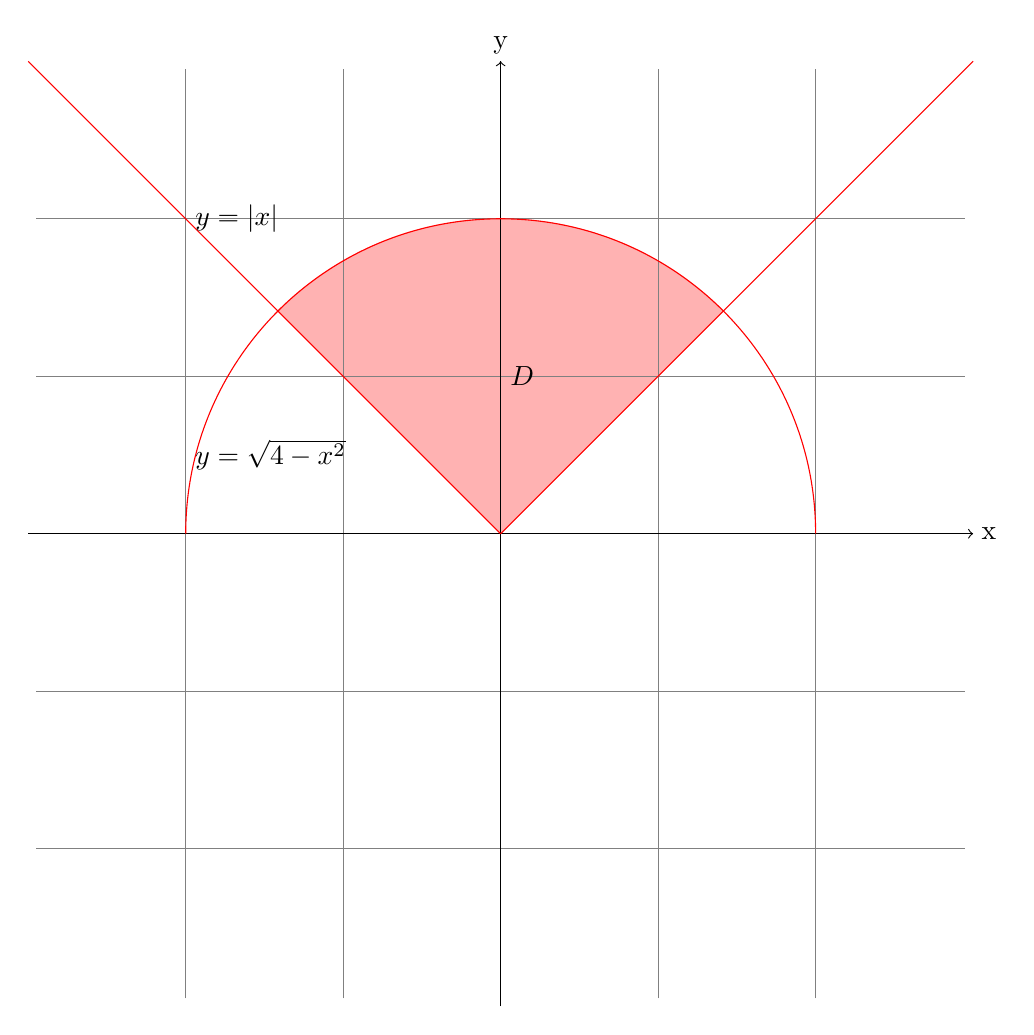
\begin{tikzpicture}
    \filldraw[color=red!30](2.828,2.828) arc (45:135:4);
    \filldraw[color=red!30](0,0) -- (2.8285, 2.8285) -- (-2.8285, 2.8285) -- cycle;
    
    \draw[step=2cm,gray,very thin] (-5.9,-5.9) grid (5.9,5.9);
    \draw (-6,0) -- (6,0);
    \draw (0,-6) -- (0,6);
    \draw[->] (-6,0) -- (6,0); 
    \draw[->] (0,-6) -- (0,6);
    \draw (0, 6.2) node {y};
    \draw (6.2, 0) node {x};
    \draw[color=red](4,0) arc (0:180:4);
    \draw[color=red](0,0) -- (-6, 6);
    \draw[color=red](0,0) -- (6, 6);
    \draw(-4,4) node[anchor=west]{$y=|x|$};
    \draw(-4,1) node[anchor=west]{$y=\sqrt{4-x^2}$};
    \draw(0,2) node[anchor=west]{$D$};
    
    
\end{tikzpicture}

    Om man skriver om til polarkoordinater er arealet av $D$ lik
    \begin{align*}
        \frac{1}{2}\int_{\frac{\pi}{4}}^{\frac{3\pi}{4}}4dr&=\frac{1}{2}\left[4r\right]_{\frac{\pi}{4}}^{\frac{3\pi}{4}}\\
        &=\pi
    \end{align*}
\end{oppgave}

\begin{oppgave}
    \begin{align*}
        \int\int_D(x-y^2)dA &= \int_0^1\int_{x^3}^{x^2}(x-y^2)dydx\\
        &=\int_0^1\left[xy-\frac{1}{3}y^3\right]_{y=x^3}^{y=x^2}dx\\
        &=\int_0^1\left(x^3-\frac{1}{3}x^6\right)-\left(x^4-\frac{1}{3}x^9\right)dx\\
        &=\frac{1}{4}-\frac{1}{21}-\frac{1}{5}+\frac{1}{30}\\
        &=\frac{1}{28}
    \end{align*}
\end{oppgave}

\begin{oppgave}
    Området er symmetrisk om $xy$-planet. Derfor kan vi forenkle regningen ved å regne ut volumet som er over $xy$-planet, og å deretter doble det. Skjæringen mellom $T$ og $xy$-planet er en sirkel med radius $1$ og senter i $(0, 1)$, la dette området kalles $D$. Den delen av $T$ som er over $D$ er da bestemt ved likningen for kulen, ettersom likningen for sylinderen ikke har en begrenset høyde. Det gir at volumet utspent av $T$ over $D$ er gitt ved
    \begin{align*}
        \int\int_D\int_0^{\sqrt{4-x^2-y^2}}dzdA.
    \end{align*}
    
    $D$ kan uttrykkes med polarkoordinater som $r(\theta )=2\sin\theta, \theta \in [0, \pi)$. Med $x=r\sin\theta$ og $y=r\cos\theta$ blir integralet slik:
    \begin{align*}
        \int_0^{\pi}\int_0^{2\sin\theta}\left(\int_0^{\sqrt{4-r^2}}dz\right)rdrd\theta &=\int_0^{\pi}\int_0^{2\sin\theta}r\sqrt{4-r^2}drd\theta.
    \end{align*}
    Med substisusjonen $u=4-r^2$ får vi $du=-2rdr$, og integralet blir
    \begin{align*}
        \int_0^{\pi}\frac{-1}{2}\int_4^{4-4\sin^2\theta}\sqrt{u}dud\theta&=\frac{-1}{2}\cdot \frac{2}{3}\int_0^\pi \left(4\cos^2\theta \right)^\frac{3}{2}-4^\frac{3}{2}d\theta
        \\&=\frac{-8}{3}\int_0^\pi |\cos^3\theta|-1d\theta
        \\&=\frac{-16}{3}\int_0^\frac{\pi}{2} \cos^3\theta d\theta+\frac{8\pi}{3}
        \\&=\frac{-16}{3}\int_0^\frac{\pi}{2} \cos\theta\cos^2\theta d\theta +\frac{8\pi}{3}
        \\&=\frac{8\pi}{3}-\frac{16}{3}\int_0^\frac{\pi}{2} \cos\theta\left( \frac{1}{2}\cos 2\theta +\frac{1}{2}\right) d\theta
        \\&=\frac{8\pi}{3}-\frac{16}{3}\left(-\sin 2\theta\cos\theta \bigg|_0^\frac{\pi}{2} -\int_0^\frac{\pi}{2} -\sin\theta \sin 2\theta d\theta\right)
        \\&=\frac{8\pi}{3}-\frac{16}{3}\int_0^\frac{\pi}{2} \sin\theta \sin 2\theta d\theta
        \\&=\frac{8\pi}{3}-\frac{8}{3}\int_0^\frac{\pi}{2}-\cos 3\theta +\cos(-\theta) d\theta
        \\&=\frac{8\pi}{3}-\frac{8}{3}\left[-\frac{1}{3}\sin 3\theta + \sin\theta \right]_0^\frac{\pi}{2}
        \\&=\frac{8\pi}{3}-\frac{8}{3}\left(\frac{1}{3} +1 -0-0\right)
        \\&=\frac{8\pi}{3}-\frac{32}{9}.
    \end{align*}
    Dette må til slutt dobles, og vi får at volumet til $T$ er $\frac{16\pi}{3}-\frac{64}{9}$.
\end{oppgave}

\end{document}